\documentclass[11pt,a4paper]{article}

\usepackage[margin=1in]{geometry}
\usepackage{amsmath,amssymb,amsthm,mathtools}
\usepackage{booktabs}
\usepackage{array}
\usepackage{graphicx}
\usepackage{xcolor}
\usepackage{enumitem}
\usepackage{microtype}
\usepackage[hidelinks,
  pdftitle={Exact-Q Finite-Setting Steering Gap Laws, Rational Polytope Certificates, and Machine-Checked Two-Copy Superactivation of PVM-Critical Two-Qubit States},
  pdfauthor={Lluis Eriksson}
]{hyperref}

\newtheorem{theorem}{Theorem}[section]
\newtheorem{proposition}[theorem]{Proposition}
\newtheorem{lemma}[theorem]{Lemma}
\newtheorem{corollary}[theorem]{Corollary}
\theoremstyle{definition}
\newtheorem{definition}[theorem]{Definition}
\theoremstyle{remark}
\newtheorem{remark}[theorem]{Remark}

\newcommand{\QQ}{\mathbb{Q}}
\newcommand{\RR}{\mathbb{R}}
\newcommand{\CC}{\mathbb{C}}
\newcommand{\ZZ}{\mathbb{Z}}
\newcommand{\NN}{\mathbb{N}}
\newcommand{\Tr}{\operatorname{Tr}}
\newcommand{\sgn}{\operatorname{sgn}}
\newcommand{\certschema}{\texttt{EPR-STEER-CERT-1.0}}
\emergencystretch=1.5em

\title{\bfseries Exact-$\QQ$ Finite-Setting Steering Gap Laws, Rational Polytope Certificates, and Machine-Checked Two-Copy Superactivation of PVM-Critical Two-Qubit States}

\author{Lluis Eriksson\thanks{Independent researcher (Sweden). Prepared with AI assistance (Google Antigravity). Code, zero-dependency Lean~4 formalization, and exact-$\QQ$ certificates (MIT license):\\ \url{https://github.com/lluiseriksson/critical-steering-certificates}.}}

\date{November 2026}

\begin{document}
\maketitle

\begin{abstract}
Einstein--Podolsky--Rosen (EPR) steering of two-qubit states exhibits sharp critical behavior at the projective-measurement (PVM) unsteerability boundary $v_c = 1/2$ of the Werner family $\rho_v = v|\Psi^-\rangle\langle\Psi^-| + (1-v)I/4$. Very recently, Zhang and Chen (\texttt{arXiv:2611.09321}, November 2026) proved that every PVM-critical entangled two-qubit state is superactivated by two copies with separable conditional states on Bob's side, while every fixed finite bound $m$ on the number of measurement settings leaves an unsteerable neighborhood around criticality. Here we turn both phenomena into exact, closed-form rational theorems over $\QQ$, backed by a zero-dependency Lean~4 formalization and a pure-stdlib zero-floating-point-trust certificate verifier (\certschema{}). First, by combining exact great-circle cell counting ($R(m) \le m(m-1) + 2$), a spherical-cap centroid rearrangement inequality ($\|\mathbf{m}_r\|_2 \le \alpha_r(1-\alpha_r)$), and Cauchy--Schwarz, we prove the universal non-asymptotic finite-setting unsteerability law $v_m^* \ge \frac{1}{2} + \frac{1}{2(m^2 - m + 1)}$ valid for \emph{every} $m \ge 1$ and \emph{every} choice of $m$ projective measurements on $S^2$---matching the exact $v_1^* = 1$ at $m=1$, coming within $1.1\%$ of optimal at $m=3$ ($4/7$ vs.\ $1/\sqrt{3}$), and establishing the quantitative $\Omega(m^{-2})$ gap law with zero hidden constants. Second, via squared-rational primal--dual steering polytope certificates across $m \in \{2,3,4,6,7,12,15\}$, we prove that the rational cuboctahedron ($m=6$, exact threshold $v_6^{\mathrm{cub}} = \sqrt{5/18} \approx 0.5270$, bracketed over $\QQ$ by a $24$-state LHS model at $v=21/40=0.525$ and a witness at $v=53/100=0.530$) strictly outperforms the Platonic icosahedron (exact threshold $v_6^{\mathrm{ico}} = (1+\sqrt{5})/6 \approx 0.5393$, $(v_6^{\mathrm{ico}})^2 = (3+\sqrt{5})/18$) in exact $6$-setting steering threshold. Third, for two copies $\rho_v^{\otimes 2}$ under partially entangled Bell measurements $|\psi_j(t)\rangle$, we derive exact closed-form partial-transpose eigenvalues $\lambda_{\min}^{\mathrm{PT}} = (1 - v^2(1+2s))/4$ (proving strict conditional separability $\lambda_{\min}^{\mathrm{PT}} \ge 1/16 > 0$ at $v=1/2$ for all $s \in [0,1]$), and construct an unconditional, zero-float exact-$\QQ$ proof of two-copy superactivation of $\rho_{1/2}^{\otimes 2}$ (extending strictly below criticality to $v = 49999/100000 < 1/2$) via a Bell sign-parity identity, a degree-$5$ sum-of-squares polynomial factorization, and the exact spherical moment $\mathbb{E}_{S^2}[x^2 y^2 z^2] = 1/105$. All $18$ foundational theorems are machine-checked in zero-dependency Lean~4 (\texttt{v4.35.0}, $0$~\texttt{sorry}, $0$~\texttt{Classical.choice}, $0$~warnings), validated against $100{,}000$-sample Haar $SO(3)\times SO(3)$ Monte Carlo ($z = 0.96$) and $40$ matrix PPT checks (error $1.11\times 10^{-16}$), and operationalized in $14$ exact-$\QQ$ certificates rejecting $46/46$ live adversarial attacks.
\end{abstract}

\section{Introduction}

Einstein--Podolsky--Rosen (EPR) steering~\cite{wiseman2007steering,cavalcanti2017quantum,uola2020quantum} occupies the strict operational hierarchy between entanglement and Bell nonlocality: a bipartite state $\rho_{AB}$ is unsteerable from Alice to Bob under a measurement set $\{M_{a|x}\}$ if Bob's unnormalized conditional states $\sigma_{a|x} = \Tr_A((M_{a|x} \otimes I)\rho_{AB})$ admit a local hidden state (LHS) decomposition $\sigma_{a|x} = \sum_\lambda p_\lambda D(a|x,\lambda)\rho_\lambda$. For the canonical two-qubit Werner family~\cite{werner1989quantum}
\begin{equation}
  \rho_v = v|\Psi^-\rangle\langle\Psi^-| + (1-v)\frac{I_4}{4}
         = \frac{1}{4}\!\left(I\otimes I - v\sum_{k=1}^3 \sigma_k \otimes \sigma_k\right),
  \qquad v \in [0, 1],
\end{equation}
entanglement begins at $v > 1/3$, whereas continuous projective-measurement (PVM) steering begins precisely at the critical threshold $v_c = 1/2$~\cite{wiseman2007steering}.

Two remarkable features of steering criticality have crystallized over the past decade and culminated in the November 2026 breakthrough of Zhang and Chen~\cite{zhang2026critical} (\texttt{arXiv:2611.09321}):
\begin{enumerate}[leftmargin=1.8em,itemsep=2pt]
  \item \textbf{Superactivation of PVM-critical states:} Building on Quintino, Brunner, and Huber~\cite{quintino2016superactivation} and Palazuelos~\cite{palazuelos2012superactivation}, Zhang and Chen~\cite{zhang2026critical} proved that \emph{every} PVM-critical entangled two-qubit state becomes steerable with two copies $\rho^{\otimes 2}$ using joint measurements whose conditional states on Bob's two qubits remain completely separable.
  \item \textbf{Finite-setting unsteerable gap:} Simultaneously, Zhang and Chen~\cite{zhang2026critical} proved qualitatively that restricting Alice to any fixed finite number $m$ of measurement settings always leaves an unsteerable neighborhood around the critical boundary.
\end{enumerate}

Despite this structural clarity, three quantitative and certification gaps remain open:
\begin{itemize}[leftmargin=1.6em,itemsep=2pt]
  \item \textbf{Non-asymptotic universal finite-$m$ gap law:} Can one prove a closed-form, zero-constant rational lower bound $v_m^* \ge \frac{1}{2} + \Delta_{\mathrm{univ}}(m)$ valid for \emph{every} $m \ge 1$ and \emph{every} configuration of $m$ projective measurements on $S^2$?
  \item \textbf{Exact-$\QQ$ primal--dual polytope thresholds:} Previous finite-$m$ steering benchmarks~\cite{saunders2010experimental,nguyen2016necessary,cavalcanti2017quantum} rely on floating-point semidefinite programming (SDP) solvers. Can both upper bounds (linear steering witnesses) and lower bounds (explicit finite LHS ensembles) be certified strictly over $\QQ$ with zero floating-point trust?
  \item \textbf{Unconditional machine-checked two-copy superactivation:} Can two-copy superactivation of $\rho_{1/2}^{\otimes 2}$ (and even strictly below $v = 1/2$)---together with exact conditional-state separability on Bob's two qubits---be certified purely in exact rational arithmetic without numerical integration or floating-point SDP relaxations?
\end{itemize}

\paragraph{Summary of Contributions.}
We resolve all three problems with exact rational algebra, a zero-dependency Lean~4 kernel ($18$ theorems), and a pure-stdlib verifier (\certschema{}):
\begin{enumerate}[leftmargin=1.8em,itemsep=2pt]
  \item \textbf{Universal Finite-$m$ Steering Gap Law (Theorem~\ref{thm:univ-gap}):} For every $m \ge 1$ and every $m$ projective axes $\{\mathbf{u}_1,\dots,\mathbf{u}_m\} \subset S^2$, $\rho_v$ is provably unsteerable for all $v \le \frac{m^2-m+2}{2(m^2-m+1)} = \frac{1}{2} + \frac{1}{2(m^2-m+1)}$, quantifying the $\Omega(m^{-2})$ gap above $v_c = 1/2$ with zero hidden constants.
  \item \textbf{Exact-$\QQ$ Polytope Duality and Cuboctahedral Supremacy (Theorem~\ref{thm:polytope}):} We establish squared-rational primal--dual steering certificates across $m \in \{2,3,4,6,7,12,15\}$, proving that at $m=6$ the rational cuboctahedron (exact threshold $v_6^{\mathrm{cub}} = \sqrt{5/18} \approx 0.5270$, with an exact primal--dual rational bracket $0.525 < \sqrt{5/18} < 0.530$) strictly outperforms the Platonic icosahedron (exact threshold $v_6^{\mathrm{ico}} = (1+\sqrt{5})/6 \approx 0.5393$, $(v_6^{\mathrm{ico}})^2 = (3+\sqrt{5})/18$).
  \item \textbf{Exact-$\QQ$ Two-Copy Superactivation with Separable Conditionals (Theorem~\ref{thm:superact}):} We derive the closed-form PPT spectrum of Bob's two-qubit conditional states ($\lambda_{\min}^{\mathrm{PT}} = (1 - v^2(1+2s))/4 \ge 1/16 > 0$ at $v=1/2$) and prove unconditionally over $\QQ$ that $\rho_v^{\otimes 2}$ violates all two-qubit LHS models at $v = 1/2$ (margin $+1199/134064$) and strictly below criticality at $v = 49999/100000 < 1/2$.
  \item \textbf{Lean~4 Formalization and \certschema{} Verifier (Theorem~\ref{thm:cert}):} All $18$ core theorems are verified in zero-dependency Lean~4 (\texttt{v4.35.0}, $0$~\texttt{sorry}, $0$~\texttt{Classical.choice}, $0$~warnings); $14$ standalone exact-$\QQ$ certificates across $4$ mutually exclusive modes pass independent verification while rejecting $46/46$ live adversarial attacks.
\end{enumerate}

\section{Preliminaries}

For Alice's projective measurement along a unit Bloch vector $\mathbf{u}_x \in S^2$ with outcomes $a \in \{-1, +1\}$ ($M_{a|x} = \frac{I + a\,\mathbf{u}_x\cdot\boldsymbol{\sigma}}{2}$), the Werner state $\rho_v$ produces Bob's unnormalized conditional states
\begin{equation}
  \sigma_{a|x} = \Tr_A\bigl((M_{a|x} \otimes I)\rho_v\bigr) = \frac{1}{2}\!\left(\frac{I - a v\,\mathbf{u}_x \cdot \boldsymbol{\sigma}}{2}\right).
\end{equation}
An $m$-setting LHS model specifies probabilities $p_\lambda > 0$ ($\sum_\lambda p_\lambda = 1$), deterministic responses $a_x^{(\lambda)} \in \{-1, +1\}$, and valid qubit hidden states $\rho_\lambda = \frac{I + \mathbf{n}^{(\lambda)}\cdot\boldsymbol{\sigma}}{2}$ ($\|\mathbf{n}^{(\lambda)}\|_2^2 \le 1$) satisfying
\begin{equation}\label{eq:lhs-def}
  \sum_{\lambda} p_\lambda \mathbf{n}^{(\lambda)} = \mathbf{0}, \qquad
  \sum_{\lambda} p_\lambda a_x^{(\lambda)} = 0, \qquad
  \sum_{\lambda} p_\lambda a_x^{(\lambda)} \mathbf{n}^{(\lambda)} = v\,\mathbf{u}_x \qquad \forall x \in \{1,\dots,m\},
\end{equation}
encoding respectively Bob's isotropic marginal $\sum_a \sigma_{a|x} = I/2$, Alice's uniform outcome probabilities $\Tr(\sigma_{\pm|x}) = 1/2$, and exact Bloch correlations (absorbing the global minus sign into $a_x^{(\lambda)} \mapsto -a_x^{(\lambda)}$). For any linear steering witness $\{\mathbf{f}_1,\dots,\mathbf{f}_m\} \subset \RR^3$ with $\sum_{x=1}^m \mathbf{u}_x \cdot \mathbf{f}_x > 0$, every LHS model obeys the Cauchy--Schwarz bound
\begin{equation}\label{eq:witness-duality}
  v \sum_{x=1}^m \mathbf{u}_x \cdot \mathbf{f}_x
  = \sum_{\lambda} p_\lambda \mathbf{n}^{(\lambda)} \cdot \left(\sum_{x=1}^m a_x^{(\lambda)} \mathbf{f}_x\right)
  \le \max_{\mathbf{a} \in \{-1,+1\}^m} \left\|\sum_{x=1}^m a_x \mathbf{f}_x\right\|_2.
\end{equation}
On two copies $\rho_v^{\otimes 2}$ distributed across $(A_1 B_1)(A_2 B_2)$, any partially entangled Bell basis on $A_1 A_2$ parameterized by rational entanglement ratio $t \in \QQ \cap [0, 1]$ ($c := \frac{1-t^2}{1+t^2}$, $s := \frac{2t}{1+t^2}$, $c^2 + s^2 = 1$),
\begin{align}\label{eq:partial-bell}
  |\psi_0(t)\rangle &= \frac{|00\rangle + t|11\rangle}{\sqrt{1+t^2}}, &
  |\psi_1(t)\rangle &= \frac{t|00\rangle - |11\rangle}{\sqrt{1+t^2}}, \notag\\
  |\psi_2(t)\rangle &= \frac{|01\rangle + t|10\rangle}{\sqrt{1+t^2}}, &
  |\psi_3(t)\rangle &= \frac{t|01\rangle - |10\rangle}{\sqrt{1+t^2}},
\end{align}
occurs with uniform probability $p_j = 1/4$ and induces Bob's conditional state
\begin{equation}\label{eq:cond-state}
  \rho_{B_1 B_2}^{(0)}(v,t)
  = \frac{1}{4}\!\Bigl(I\otimes I - v c\,(Z\otimes I + I\otimes Z) + v^2\bigl(s\,X\otimes X - s\,Y\otimes Y + Z\otimes Z\bigr)\Bigr),
\end{equation}
with $\rho_{B_1 B_2}^{(1,2,3)}$ obtained from the Bell sign patterns $(+s,-s,+1)$, $(-s,+s,+1)$, $(+s,+s,-1)$, $(-s,-s,-1)$ and local signs $(+c,+c)$, $(-c,-c)$, $(+c,-c)$, $(-c,+c)$.

\section{Main Theorems}

\subsection{Universal Exact-\texorpdfstring{$\QQ$}{Q} Finite-\texorpdfstring{$m$}{m} Steering Gap Law}

\begin{theorem}[Universal Finite-$m$ Unsteerability Radius]\label{thm:univ-gap}
For every integer $m \ge 1$ and \emph{every} configuration of $m$ projective measurement axes $\{\mathbf{u}_1,\dots,\mathbf{u}_m\} \subset S^2$, the two-qubit Werner state $\rho_v$ is unsteerable for all
\begin{equation}\label{eq:univ-gap}
  v \le v_{\mathrm{univ}}(m) := \frac{m(m-1) + 2}{2\bigl(m(m-1) + 1\bigr)} = \frac{1}{2} + \frac{1}{2(m^2 - m + 1)},
\end{equation}
admitting an explicit finite LHS model with at most $R_{\max}(m) = m(m-1) + 2$ pure hidden states at the critical radius $v = 1/(2S) \ge v_{\mathrm{univ}}(m)$ (and for every $v \le v_{\mathrm{univ}}(m)$ via convex mixing with the isotropic $v=0$ model, using at most $2 R_{\max}(m)$ deterministic response--state pairs).
In particular, $v_{\mathrm{univ}}(1) = 1$ (exact), $v_{\mathrm{univ}}(m)$ is strictly decreasing in $m$, and every $m$-setting PVM protocol leaves a provably unsteerable neighborhood of width $\Delta_{\mathrm{univ}}(m) = \frac{1}{2(m^2-m+1)} = \Omega(m^{-2})$ strictly above the critical boundary $v_c = 1/2$.
\end{theorem}

\begin{proof}
The $m$ great circles $C_x = \{\mathbf{n} \in S^2 : \mathbf{n}\cdot \mathbf{u}_x = 0\}$ ($x=1,\dots,m$) partition $S^2 \setminus \bigcup_x C_x$ into $R$ open spherical cells $D_1,\dots,D_R$. Inductively, the $k$-th distinct great circle intersects the preceding $k-1$ circles in at most $2(k-1)$ points, dividing itself into at most $2(k-1)$ arcs that each split at most one region, so $R \le R_{\max}(m) = 2 + \sum_{k=2}^m 2(k-1) = m(m-1) + 2$ (Lean~4 Theorem~1).

On each cell $D_r$ of fractional area $\alpha_r := \frac{1}{4\pi}\int_{D_r} d\Omega > 0$ ($\sum_{r=1}^R \alpha_r = 1$), the sign vector $\mathbf{a}^{(r)} = (\sgn(\mathbf{n}\cdot \mathbf{u}_x))_{x=1}^m \in \{-1,+1\}^m$ is constant. Define the cell centroid $\mathbf{m}_r := \frac{1}{4\pi}\int_{D_r} \mathbf{n}\,d\Omega$, its norm $s_r := \|\mathbf{m}_r\|_2$, and total norm $S := \sum_{r=1}^R s_r$. Because $\frac{1}{4\pi}\int_{S^2} \sgn(\mathbf{n}\cdot \mathbf{u}_x)\mathbf{n}\,d\Omega = \frac{1}{2}\mathbf{u}_x$, $\int_{S^2}\mathbf{n}\,d\Omega = \mathbf{0}$, and antipodal symmetry pairs each cell $D_r$ with $-D_r$ of equal centroid norm $s_{-r} = s_r$ and negated sign vector $\mathbf{a}^{(-r)} = -\mathbf{a}^{(r)}$, setting $p_r := s_r / S$ and pure Bloch vectors $\hat{\mathbf{n}}_r := \mathbf{m}_r / s_r \in S^2$ (for $s_r > 0$) yields a valid $R$-state LHS model satisfying $\sum_r p_r a_x^{(r)} = 0$, $\sum_r p_r \hat{\mathbf{n}}_r = \mathbf{0}$, and $\sum_r p_r a_x^{(r)} \hat{\mathbf{n}}_r = \frac{1}{2S}\mathbf{u}_x$ for all $x=1,\dots,m$, certifying unsteerability for all $v \le \frac{1}{2S}$.

To upper-bound $s_r$, set $\hat{\mathbf{e}}_r = \mathbf{m}_r / s_r \in S^2$ and let $C_r = \{\mathbf{n} \in S^2 : \mathbf{n}\cdot \hat{\mathbf{e}}_r \ge t_r\}$ be the polar cap centered at $\hat{\mathbf{e}}_r$ of equal fractional area $\alpha_r = (1 - t_r)/2$ (so $t_r = 1 - 2\alpha_r$). Since $\mathbf{n}\cdot\hat{\mathbf{e}}_r \ge t_r$ on $C_r \setminus D_r$ and $\mathbf{n}\cdot\hat{\mathbf{e}}_r \le t_r$ on $D_r \setminus C_r$ while $\operatorname{Area}(C_r\setminus D_r) = \operatorname{Area}(D_r\setminus C_r)$, rearrangement yields
\[
  s_r = \frac{1}{4\pi}\int_{D_r} (\mathbf{n}\cdot \hat{\mathbf{e}}_r)\,d\Omega
      \le \frac{1}{4\pi}\int_{C_r} (\mathbf{n}\cdot \hat{\mathbf{e}}_r)\,d\Omega
      = \frac{1}{2}\int_{t_r}^1 z\,dz = \frac{1 - t_r^2}{4} = \alpha_r(1 - \alpha_r),
\]
whose cleared-denominator algebraic identity is verified in Lean~4 (Theorem~2). Summing over $r=1,\dots,R$ and applying Cauchy--Schwarz $\sum_{r=1}^R \alpha_r^2 \ge \frac{1}{R}(\sum_{r=1}^R \alpha_r)^2 = \frac{1}{R}$ (Lean~4 Theorems~3--4) gives
\[
  S = \sum_{r=1}^R s_r \le \sum_{r=1}^R \alpha_r(1-\alpha_r) = 1 - \sum_{r=1}^R \alpha_r^2 \le 1 - \frac{1}{R} \le 1 - \frac{1}{R_{\max}(m)} = \frac{R_{\max}(m)-1}{R_{\max}(m)},
\]
whence $v \le \frac{1}{2S} \ge \frac{R_{\max}(m)}{2(R_{\max}(m)-1)} = \frac{1}{2} + \frac{1}{2(m^2-m+1)}$. Strict positivity above $1/2$, monotonicity in $m$, and exact tightness $v_{\mathrm{univ}}(1)=1$ are proved in Lean~4 (Theorems~5--7).
\end{proof}

\subsection{Exact-\texorpdfstring{$\QQ$}{Q} Polytope Steering Duality and Cuboctahedral Supremacy}

\begin{theorem}[Squared-Rational Polytope Certificates and Cuboctahedral Supremacy]\label{thm:polytope}
Let $\mathbf{w}_1,\dots,\mathbf{w}_m \in \QQ^3$ satisfy $\|\mathbf{w}_x\|_2^2 = N_u \in \QQ_{>0}$ for all $x$ (defining unit axes $\mathbf{u}_x = \mathbf{w}_x / \sqrt{N_u} \in S^2$).
\begin{enumerate}[leftmargin=1.8em,itemsep=2pt]
  \item \textbf{Zero-Square-Root Primal--Dual Certification:} For any rational witness $\{\mathbf{f}_x\} \subset \QQ^3$ with $\sum_x \mathbf{w}_x\cdot\mathbf{f}_x > 0$, $\rho_v$ is $m$-setting steerable whenever
  \begin{equation}\label{eq:sq-witness}
    \frac{v^2}{N_u}\!\left(\sum_{x=1}^m \mathbf{w}_x\cdot\mathbf{f}_x\right)^2 > \max_{\mathbf{a}\in\{-1,+1\}^m}\left\|\sum_{x=1}^m a_x \mathbf{f}_x\right\|_2^2 \quad\text{in }\QQ.
  \end{equation}
  Conversely, any rational ensemble $\{(p_\lambda, \mathbf{a}^{(\lambda)}, \mathbf{b}^{(\lambda)})\}$ with $p_\lambda > 0$, $\sum p_\lambda = 1$, $\|\mathbf{b}^{(\lambda)}\|_2^2 \le N_u$, $\sum p_\lambda \mathbf{b}^{(\lambda)} = \mathbf{0}$, $\sum p_\lambda a_x^{(\lambda)} = 0$, and $\sum p_\lambda a_x^{(\lambda)} \mathbf{b}^{(\lambda)} = v\mathbf{w}_x$ ($\forall x$) certifies $m$-setting unsteerability of $\rho_v$ strictly over $\QQ$.
  \item \textbf{Exact Cuboctahedral Threshold and Supremacy over the Icosahedron ($m=6$):} For the $6$-axis rational cuboctahedron $\mathbf{w}_x \in \{(1,\pm 1,0),(1,0,\pm 1),(0,1,\pm 1)\}$ ($N_u = 2$), the exact $6$-setting steering threshold is $v_6^{\mathrm{cub}} = \sqrt{5/18} \approx 0.527046$, attained on both sides by the canonical witness $\mathbf{f}_x = \mathbf{w}_x$ ($\max_{\mathbf{a}}\|\sum a_x\mathbf{w}_x\|_2^2 = 20$) and the uniform $24$-state LHS ensemble of signed permutations of $\alpha(2,1,0)$ ($\|\mathbf{b}\|_2^2 = 5\alpha^2 \le 2$, $v = \frac{5}{6}\alpha$). By contrast, for the $6$-axis Platonic icosahedron, the exact $6$-setting steering threshold is $v_6^{\mathrm{ico}} = \frac{1+\sqrt{5}}{6} \approx 0.539345$ ($(v_6^{\mathrm{ico}})^2 = \frac{3+\sqrt{5}}{18}$), attained on both sides by the canonical witness and the uniform $12$-state icosahedral-vertex LHS ensemble. Thus the rational cuboctahedron strictly beats the Platonic icosahedron in exact $6$-setting steering threshold, since $\frac{5}{18} < \frac{3+\sqrt{5}}{18} \iff (5-3)^2 < 5 \iff 4 < 5$ (Lean~4 Theorem~8).
\end{enumerate}
\end{theorem}

\begin{proof}
Part~1 follows directly from squaring~\eqref{eq:witness-duality} and rescaling $\mathbf{n}^{(\lambda)} = \mathbf{b}^{(\lambda)}/\sqrt{N_u}$ in~\eqref{eq:lhs-def}. For Part~2, summing $6$ cuboctahedron vectors with optimal signs gives $\|(4,2,0)\|_2^2 = 20$, so $(v_6^{\mathrm{cub}})^2 = \frac{2 \cdot 20}{12^2} = \frac{5}{18}$. Conversely, for the $24$ signed permutations $\mathbf{b}^{(\lambda)}$ of $\alpha(2,1,0)$ with $p_\lambda = 1/24$ and $a_x^{(\lambda)} = \sgn(\mathbf{w}_x\cdot\mathbf{b}^{(\lambda)})$, antipodal symmetry gives $\sum_\lambda p_\lambda \mathbf{b}^{(\lambda)} = \mathbf{0}$ and $\sum_\lambda p_\lambda a_x^{(\lambda)} = 0$, while $\sum_{\lambda=1}^{24}|\mathbf{w}_x\cdot\mathbf{b}^{(\lambda)}| = 40\alpha$ yields $\frac{1}{24}\sum_\lambda a_x^{(\lambda)}\mathbf{b}^{(\lambda)} = \frac{5}{6}\alpha\mathbf{w}_x$. Taking $\alpha = \sqrt{2/5}$ matches $\sqrt{5/18}$ identically, while the rational choice $\alpha = 63/100$ ($5\alpha^2 = 19845/10000 \le 2$) certifies $v = 21/40 = 0.525$. For the $6$ icosahedral axes $\mathbf{u}_x \in \frac{1}{\sqrt{1+\varphi^2}}\{(0,\pm 1,\pm\varphi)\text{ cyclic}\}$ ($\varphi = \frac{1+\sqrt{5}}{2}$), every pair of distinct axes satisfies $|\mathbf{u}_x\cdot\mathbf{u}_y| = 1/\sqrt{5}$. Aligning signs with one vertex $\mathbf{u}_0$ and its $5$ nearest neighbors gives $\|\sum_{x=1}^6 a_x \mathbf{u}_x\|_2 = 1 + \sqrt{5}$ (squared norm $6 + 2\sqrt{5}$), yielding $v_6^{\mathrm{ico}} = \frac{1+\sqrt{5}}{6}$ and $(v_6^{\mathrm{ico}})^2 = \frac{6+2\sqrt{5}}{36} = \frac{3+\sqrt{5}}{18}$; conversely, the uniform $12$-state LHS ensemble $\mathbf{n}^{(\lambda)} = \pm\mathbf{u}_y$ ($p_\lambda = 1/12$, $a_x^{(\lambda)} = \sgn(\mathbf{u}_x\cdot\mathbf{n}^{(\lambda)})$) reproduces $\frac{1}{6}(1 + 5\cdot\frac{1}{\sqrt{5}})\mathbf{u}_x = \frac{1+\sqrt{5}}{6}\mathbf{u}_x$ with zero marginals, establishing $v_6^{\mathrm{ico}} = \frac{1+\sqrt{5}}{6}$ as the exact $6$-setting threshold. Comparing squared thresholds yields $\frac{5}{18} < \frac{3+\sqrt{5}}{18} \iff 2 < \sqrt{5} \iff 4 < 5$ (Lean~4 Theorem~8).
\end{proof}

\subsection{Exact-\texorpdfstring{$\QQ$}{Q} Two-Copy Superactivation with Strictly Separable Conditionals}

\begin{theorem}[Conditional Separability and Unconditional Exact-$\QQ$ Two-Copy Superactivation]\label{thm:superact}
Consider two copies $\rho_v^{\otimes 2}$ of the two-qubit Werner state.
\begin{enumerate}[leftmargin=1.8em,itemsep=2pt]
  \item \textbf{Exact Rational PPT Spectrum of Conditional States:} Under the partially entangled Bell basis~\eqref{eq:partial-bell} with $c = \frac{1-t^2}{1+t^2}$ and $s = \frac{2t}{1+t^2}$ ($t \in [0,1]$), the four exact eigenvalues of Bob's partial-transposed conditional state $\rho_{B_1 B_2}^{(j)\,\mathsf{T}_2}$ are
  \begin{equation}\label{eq:ppt-eigs}
    \lambda_{1,2} = \frac{1 \mp 2vc + v^2}{4}, \qquad
    \lambda_{3,4} = \frac{1 - v^2 \pm 2v^2 s}{4}.
  \end{equation}
  By the Peres--Horodecki criterion~\cite{peres1996separability}, all four conditional states on $B_1 B_2$ are separable if and only if $v^2(1 + 2s) \le 1$. In particular, for all $v \le 1/\sqrt{3}$ (including $v \le 1/2$), every conditional state is separable for all $s \in [0,1]$, with $\lambda_{\min}^{\mathrm{PT}} \ge 1/16 > 0$ at $v = 1/2$ (Lean~4 Theorem~18).
  \item \textbf{Unconditional Exact-$\QQ$ Two-Copy Superactivation:} Define the two-copy steering functional $W_\gamma$ ($\gamma \in \QQ_{>0}$) combining local WJD single-copy witnesses on copies $1$ and $2$ (weight $\gamma$) with the $SO(3)\times SO(3)$-averaged full Bell-basis correlation witness ($t=s=1$). Its quantum value on $\rho_v^{\otimes 2}$ is $Q_\gamma(v) = 2\gamma v + 3 v^2$, while \emph{every} two-qubit LHS model (with arbitrary separable or entangled hidden states $\sigma_\lambda$ on $B_1 B_2$) satisfies the exact rational upper bound
  \begin{equation}\label{eq:superact-ub}
    L_\gamma \le L_\gamma^{\mathrm{ub}} := \frac{5167}{7056} + \gamma + \frac{1}{\gamma}.
  \end{equation}
  At $\gamma = 114$, $Q_{114}(1/2) - L_{114}^{\mathrm{ub}} = \frac{1199}{134064} > 0$, certifying exact-$\QQ$ two-copy superactivation of the PVM-critical state $\rho_{1/2}^{\otimes 2}$, and extending strictly below criticality to $v = \frac{49999}{100000} < \frac{1}{2}$ (Lean~4 Theorem~17).
\end{enumerate}
\end{theorem}

\begin{proof}
For Part~1, partial transposition on $B_2$ sends $Y \mapsto -Y$ in~\eqref{eq:cond-state}, yielding $\rho_{B_1 B_2}^{(0)\,\mathsf{T}_2}$ block-diagonal in the computational basis $\{|00\rangle,|11\rangle\} \oplus \{|01\rangle,|10\rangle\}$ with eigenvalues~\eqref{eq:ppt-eigs}; the other outcomes $j=1,2,3$ are locally unitarily equivalent, so all four share the identical spectrum~\eqref{eq:ppt-eigs}. Since $1 - 2vc + v^2 \ge (1-v)^2 \ge 0$, PPT holds iff $\lambda_4 = (1 - v^2(1+2s))/4 \ge 0$.

For Part~2, on $\rho_v^{\otimes 2}$ each local WJD witness scores $v$ (total $2\gamma v$) and the full Bell-basis correlation witness $F_j = \Tr(T_j^\top (R_1^\top\boldsymbol{\sigma}_1 \otimes R_2^\top\boldsymbol{\sigma}_2))$ scores $v^2\Tr(T_j^\top T_j) = 3 v^2$, giving $Q_\gamma(v) = 2\gamma v + 3v^2$. For any LHS model, convexity restricts the maximum to pure two-qubit hidden states $|\phi\rangle \in \CC^4$. By $SO(3)\times SO(3)$ invariance and the Schmidt decomposition, we may set $|\phi_q\rangle = \cos q|00\rangle + \sin q|11\rangle$ ($q \in [0,\pi/4]$), which has local Bloch norms $\|\mathbf{b}_1\|_2 = \|\mathbf{b}_2\|_2 = \cos 2q$ and correlation matrix $C_B = \mathrm{diag}(\sin 2q, -\sin 2q, 1) = C_{\mathrm{prod}} + (\sin 2q) C_{\mathrm{ent}}$, where $C_{\mathrm{prod}} = \mathrm{diag}(0,0,1)$ and $C_{\mathrm{ent}} = \mathrm{diag}(1,-1,0)$. Thus the local term equals $\frac{\gamma}{2}(\cos 2q + \cos 2q) = \gamma\cos 2q$, while subadditivity of $\max_j$ gives
\[
  L_{\mathrm{joint}}(q) \le L_{\mathrm{joint}}(0) + (\sin 2q)\,\mathbb{E}_{R_1,R_2}\!\Bigl[\max_{j=0..3} X_j(R_1^\top C_{\mathrm{ent}} R_2)\Bigr].
\]
For the entangled remainder $B = R_1^\top C_{\mathrm{ent}} R_2$, the four outcomes $X_j(B)$ sum to $0$ and obey $\sum_{j=0}^3 X_j(B)^2 = 4(B_{00}^2 + B_{11}^2 + B_{22}^2)$ (Lean~4 Theorem~15). By the zero-sum Cauchy--Schwarz bound $4 X_k^2 \le 3\sum_{j=0}^3 X_j^2$ (Lean~4 Theorem~14) and Jensen's inequality,
\[
  \mathbb{E}\!\Bigl[\max_j X_j(B)\Bigr] \le \sqrt{3\,\mathbb{E}[B_{00}^2 + B_{11}^2 + B_{22}^2]} = \sqrt{3 \cdot 3 \cdot \frac{\|C_{\mathrm{ent}}\|_F^2}{9}} = \sqrt{2}.
\]
For the product baseline $q=0$, let $\mathbf{u} = R_1^\top \hat{z}, \mathbf{v} = R_2^\top \hat{z} \sim \mathrm{Unif}(S^2)$ independently and set $p_1 = |u_1 v_1|, p_2 = |u_2 v_2|, p_3 = |u_3 v_3|$ ($\sum p_i \le \|\mathbf{u}\|_2\|\mathbf{v}\|_2 = 1$). Because the four Bell sign patterns have sign-product $-1$, our exact Bell sign-parity identities (Lean~4 Theorems~9--10) give $\max_j X_j(A) = p_1+p_2+p_3$ when $\sgn(u_1 v_1 u_2 v_2 u_3 v_3) = -1$ and $p_1+p_2+p_3 - 2\min(p_1,p_2,p_3)$ when $+1$, each with exact probability $1/2$ by octant symmetry. Hence
\[
  L_{\mathrm{joint}}(0) = \mathbb{E}[p_1+p_2+p_3] - \mathbb{E}[\min(p_1,p_2,p_3)] = \frac{3}{4} - \mathbb{E}[\min(p_1,p_2,p_3)].
\]
By our degree-$5$ sum-of-squares factorization $256 - 3125 p(1-p)^4 = (5p-1)^2\bigl(16 + (1-p)(240 - 325p + 125p^2)\bigr) \ge 0$ with $4(240 - 325p + 125p^2) = 5((10p-13)^2 + 23) > 0$, we prove $3125\,p_1^2 p_2^2 p_3^2 \le 16\,\min(p_1,p_2,p_3)$ pointwise (Lean~4 Theorems~11--13). Taking expectations with the exact spherical moment $\mathbb{E}_{S^2}[x^2 y^2 z^2] = 1/105$ yields $\mathbb{E}[\min(p_1,p_2,p_3)] \ge \frac{3125}{16}\cdot\frac{1}{105^2} = \frac{125}{7056}$ and thus $L_{\mathrm{joint}}(0) \le \frac{3}{4} - \frac{125}{7056} = \frac{5167}{7056}$. Finally, 2D Cauchy--Schwarz and Lean~4 Theorem~16 give $\gamma\cos 2q + \sqrt{2}\sin 2q \le \sqrt{\gamma^2 + 2} < \gamma + \frac{1}{\gamma}$, establishing~\eqref{eq:superact-ub}. Evaluating~\eqref{eq:superact-ub} at $\gamma = 114$ proves strict superactivation at $v = 1/2$ and $v = 49999/100000$ (Lean~4 Theorem~17).
\end{proof}

\subsection{Zero-Floating-Point-Trust \texorpdfstring{\certschema{}}{EPR-STEER-CERT-1.0} Soundness}

\begin{theorem}[Soundness and Primal--Dual Exclusivity of \certschema{}]\label{thm:cert}
Every accepted \certschema{} certificate is verified solely in exact $\QQ$ arithmetic across four mutually exclusive modes: \texttt{finite\_m\_steering\_witness} (exhaustively evaluating all $2^{m-1}$ sign patterns), \texttt{finite\_m\_lhs\_model} (verifying probability normalization, Bloch-ball validity $\|\mathbf{b}^{(\lambda)}\|_2^2 \le N_u$, Bob's isotropic marginal $\sum p_\lambda \mathbf{b}^{(\lambda)} = \mathbf{0}$, Alice's uniform marginals $\sum p_\lambda a_x^{(\lambda)} = 0$, and exact correlations), \texttt{universal\_finite\_m\_gap} (replaying Theorem~\ref{thm:univ-gap}), and \texttt{two\_copy\_superactivation} (enforcing single-copy PVM unsteerability $v \le 1/2$ alongside both parts of Theorem~\ref{thm:superact}). By the $3$D Cauchy--Schwarz weak duality~\eqref{eq:witness-duality} (Lean~4 Theorem~18), no pair $(v, \{\mathbf{u}_x\})$ can simultaneously admit a valid \texttt{finite\_m\_steering\_witness} and a valid \texttt{finite\_m\_lhs\_model} (or \texttt{universal\_finite\_m\_gap}) certificate.
\end{theorem}

\begin{proof}
Suppose $(v, \{\mathbf{u}_x\})$ admits both a valid \texttt{finite\_m\_lhs\_model} certificate $\{(p_\lambda, \mathbf{a}^{(\lambda)}, \mathbf{b}^{(\lambda)})\}$ and a valid \texttt{finite\_m\_steering\_witness} certificate $\{\mathbf{f}_x\}$. Applying the $3$D Lagrange--Cauchy--Schwarz inequality (Lean~4 Theorem~18) to each hidden state $\mathbf{n}^{(\lambda)} = \mathbf{b}^{(\lambda)}/\sqrt{N_u}$ ($\|\mathbf{n}^{(\lambda)}\|_2 \le 1$) yields $S_Q = \frac{v}{\sqrt{N_u}}\sum_x \mathbf{w}_x\cdot\mathbf{f}_x \le L_{\mathrm{LHS}}$, contradicting $S_Q^2 > L_{\mathrm{LHS}}^2$. The same contradiction holds against \texttt{universal\_finite\_m\_gap} via Theorem~\ref{thm:univ-gap}.
\end{proof}

\section{Zero-Dependency Lean~4 Kernel and Exact-\texorpdfstring{$\QQ$}{Q} Verifier}

All $18$ algebraic, combinatorial, SOS, and duality theorems underlying Theorems~\ref{thm:univ-gap}--\ref{thm:cert} are formalized in \texttt{lean/CriticalSteering.lean} using pure Lean~4~\cite{demoura2021lean4} (\texttt{leanprover/lean4:v4.35.0}) with \emph{zero} external dependencies, $0$~\texttt{sorry}, $0$~\texttt{Classical.choice}, and $0$~warnings (verified by \texttt{lean/AuditAxioms.lean}). Table~\ref{tab:lean} catalogs all $18$ theorems.

\begin{remark}[Transparent Formalization Scope]
Our Lean~4 kernel formally verifies the entire discrete, algebraic, SOS, and rational-arithmetic backbone of Theorems~\ref{thm:univ-gap}--\ref{thm:cert}: great-circle region counting, the cap-centroid algebraic identity, discrete Cauchy--Schwarz, the universal gap bound and strict monotonicity, cuboctahedral supremacy ($4 < 5$), both Bell sign-parity identities, the degree-$5$ SOS factorization $256 - 3125 p(1-p)^4$ and cubic factor positivity, the cleared-denominator bound $3125 p_1^2 p_2^2 p_3^2 \le 16 p_1 D^5$, the zero-sum four-variable Cauchy--Schwarz and four-squares identities, the rational rigidity envelope $\sqrt{\gamma^2+2} < \gamma + 1/\gamma$, exact superactivation at $v=1/2$ and $v=49999/100000$, PPT conditional separability, and the $3$D Lagrange--Cauchy--Schwarz duality bound. The continuous spherical rearrangement integral, Haar averaging of $\mathbb{E}_{S^2}[x^2 y^2 z^2] = 1/105$, and Schmidt decomposition are proved analytically in Section~3 and independently validated numerically in Section~5.
\end{remark}

\begin{table}[t]
\centering
\caption{All $18$ machine-checked theorems in \texttt{lean/CriticalSteering.lean} (Lean~4 \texttt{v4.35.0}, zero external dependencies, $0$~\texttt{sorry}, $0$~\texttt{Classical.choice}, $0$~warnings).}
\label{tab:lean}
\resizebox{\textwidth}{!}{%
\begin{tabular}{@{}rll@{}}
\toprule
\# & Lean~4 Theorem Identifier & Formalized Mathematical Statement \\
\midrule
1 & \texttt{great\_circle\_regions\_closed\_form} & $R(m) = m(m-1) + 2$ for all $m \ge 1$ \\
2 & \texttt{cap\_centroid\_area\_identity} & $D^2 - (D-2a)^2 = 4a(D-a)$ (cap centroid identity) \\
3 & \texttt{discrete\_cauchy\_schwarz\_nonneg} & $(\sum a_r)^2 \le R \sum a_r^2$ over \texttt{List Int} \\
4 & \texttt{universal\_finite\_m\_gap\_bound} & $R_{\max} S_{\mathrm{num}} \le (R_{\max}-1) D^2$ (Theorem~\ref{thm:univ-gap}) \\
5 & \texttt{finite\_m\_gap\_strictly\_above\_half} & $0 < m(m-1)+1 < m(m-1)+2$ ($v_{\mathrm{univ}} > 1/2$) \\
6 & \texttt{finite\_m\_gap\_monotone} & $1 \le m_1 < m_2 \implies v_{\mathrm{univ}}(m_2) < v_{\mathrm{univ}}(m_1)$ (strict) \\
7 & \texttt{finite\_m\_single\_setting\_exact\_one} & $R(1) = 2(R(1)-1)$ ($v_{\mathrm{univ}}(1) = 1$ exact) \\
8 & \texttt{cuboctahedron\_beats\_icosahedron} & $(5 - 3)^2 < 5$ ($5/18 < (3+\sqrt{5})/18 \iff v_6^{\mathrm{cub}} < v_6^{\mathrm{ico}}$) \\
9 & \texttt{bell\_sign\_parity\_odd\_neg} & Odd-sign Bell max $= p_1 + p_2 + p_3$ \\
10 & \texttt{bell\_sign\_parity\_even\_neg} & Even-sign Bell max $= p_1 + p_2 + p_3 - 2\min(p_1,p_2,p_3)$ \\
11 & \texttt{sos\_poly\_256\_minus\_3125\_identity} & $256 D^5 - 3125 a(D-a)^4 = (5a-D)^2(\cdots)$ \\
12 & \texttt{sos\_cubic\_factor\_strictly\_pos} & $240 D^2 - 325 a D + 125 a^2 \ge 0$ via SOS \\
13 & \texttt{sos\_min\_lower\_bound\_cleared} & $3125 (p_1 p_2 p_3)^2 \le 16 p_1 D^5$ ($p_1+p_2+p_3 \le D$) \\
14 & \texttt{zero\_sum\_four\_cauchy\_schwarz} & $\sum_{j=0}^3 x_j = 0 \implies 4 x_0^2 \le 3\sum_{j=0}^3 x_j^2$ \\
15 & \texttt{bell\_four\_squares\_identity} & $\sum_{\text{Bell signs}}(\pm a \pm b \pm c)^2 = 4(a^2+b^2+c^2)$ \\
16 & \texttt{rigidity\_envelope\_rational\_upper} & $(g_n^2 + 2g_d^2) g_n^2 < (g_n^2 + g_d^2)^2$ ($\sqrt{\gamma^2+2} < \gamma + 1/\gamma$) \\
17 & \texttt{two\_copy\_superactivation\_at\_and\_below\_half} & $Q_{114}(v) > L_{114}^{\mathrm{ub}}$ at $v=1/2$ and $v=49999/100000$ \\
18 & \texttt{ppt\_conditional\_separability\_and\_witness\_duality} & $\lambda_{\min}^{\mathrm{PT}}(1/2, s) \ge 1/16$ and $3$D Cauchy--Schwarz $(\mathbf{n}\cdot\mathbf{f})^2 \le \|\mathbf{n}\|^2\|\mathbf{f}\|^2$ \\
\bottomrule
\end{tabular}}
\end{table}

\paragraph{Zero-Float Verifier (\certschema{}).}
\texttt{src/steering\_certifier.py} imports strictly Python stdlib (\texttt{fractions.\allowbreak Fraction}, \texttt{math}, \texttt{re}), enforcing strict recursive type whitelisting, single-line ASCII identifier hygiene on \texttt{cert\_id}, exact dictionary key sets, an anchored ASCII canonical rational parser, distinct projective measurement axes (rejecting duplicates and antipodal axes), Bloch-ball state validity, exhaustive sign-pattern checking, and all four theorem replays.

\section{Computational Experiments and Adversarial Red-Teaming}

All four experiments reproduce deterministically in $<5$\,s via \texttt{scripts/run\_\allowbreak all\_\allowbreak experiments.py} and pass full Gate-2 verification via \texttt{scripts/verify\_all.py}.

\paragraph{Experiment 1: Atlas of $14$ Exact-$\QQ$ Certificates.}
Table~\ref{tab:certs} summarizes all $14$ independently verified \certschema{} certificates spanning all four modes. Notably, \texttt{lhs\_m6\_\allowbreak cuboctahedron\_v525} ($24$ rational hidden states at $v = 21/40 = 0.525$) and \texttt{witness\_m6\_\allowbreak cuboctahedron\_v53} ($v = 53/100 = 0.530$) bracket the exact cuboctahedral threshold $\sqrt{5/18} \approx 0.527046$ from both sides strictly over $\QQ$; \texttt{univ\_gap\_m100\_\allowbreak v4951\_9901} certifies $100$-setting unsteerability strictly above $1/2$ in $0.10$\,ms; and \texttt{superact\_two\_\allowbreak copy\_v\_half} and \texttt{superact\_two\_\allowbreak copy\_below\_half} certify exact-$\QQ$ two-copy superactivation at $v = 1/2$ and $v = 49999/100000$ in $0.18$--$0.23$\,ms.

\begin{table}[t]
\centering
\caption{Experiment~1: $14$ independently verified zero-float \certschema{} certificates across all four modes (exact JSON files archived in \texttt{results/certificates/*.cert.json}).}
\label{tab:certs}
\resizebox{\textwidth}{!}{%
\begin{tabular}{@{}rlllrrlr@{}}
\toprule
\# & Certificate ID & Mode & Verdict & $m$ & Exact $v \in \QQ$ & Float & ms \\
\midrule
C1 & \texttt{witness\_m2\_square\_v71} & \texttt{finite\_m\_steering\_witness} & \texttt{STEERABLE} & $2$ & $71/100$ & $0.71000$ & $1.50$ \\
C2 & \texttt{witness\_m3\_octahedron\_v58} & \texttt{finite\_m\_steering\_witness} & \texttt{STEERABLE} & $3$ & $29/50$ & $0.58000$ & $0.30$ \\
C3 & \texttt{witness\_m6\_cuboctahedron\_v53} & \texttt{finite\_m\_steering\_witness} & \texttt{STEERABLE} & $6$ & $53/100$ & $0.53000$ & $0.98$ \\
C4 & \texttt{witness\_m12\_pyth221\_v56} & \texttt{finite\_m\_steering\_witness} & \texttt{STEERABLE} & $12$ & $14/25$ & $0.56000$ & $50.52$ \\
C5 & \texttt{witness\_m15\_oct\_pyth221\_v52} & \texttt{finite\_m\_steering\_witness} & \texttt{STEERABLE} & $15$ & $13/25$ & $0.52000$ & $489.03$ \\
C6 & \texttt{lhs\_m2\_square\_v70} & \texttt{finite\_m\_lhs\_model} & \texttt{UNSTEERABLE\_LHS} & $2$ & $7/10$ & $0.70000$ & $0.36$ \\
C7 & \texttt{lhs\_m3\_octahedron\_v57} & \texttt{finite\_m\_lhs\_model} & \texttt{UNSTEERABLE\_LHS} & $3$ & $57/100$ & $0.57000$ & $0.64$ \\
C8 & \texttt{lhs\_m4\_cube\_diag\_v57} & \texttt{finite\_m\_lhs\_model} & \texttt{UNSTEERABLE\_LHS} & $4$ & $57/100$ & $0.57000$ & $0.46$ \\
C9 & \texttt{lhs\_m6\_cuboctahedron\_v525} & \texttt{finite\_m\_lhs\_model} & \texttt{UNSTEERABLE\_LHS} & $6$ & $21/40$ & $0.52500$ & $1.74$ \\
C10 & \texttt{univ\_gap\_m3\_v4\_7} & \texttt{universal\_finite\_m\_gap} & \texttt{UNIV\_UNSTEERABLE} & $3$ & $4/7$ & $0.57143$ & $0.12$ \\
C11 & \texttt{univ\_gap\_m6\_v16\_31} & \texttt{universal\_finite\_m\_gap} & \texttt{UNIV\_UNSTEERABLE} & $6$ & $16/31$ & $0.51613$ & $0.16$ \\
C12 & \texttt{univ\_gap\_m100\_v4951\_9901} & \texttt{universal\_finite\_m\_gap} & \texttt{UNIV\_UNSTEERABLE} & $100$ & $4951/9901$ & $0.50005$ & $0.10$ \\
C13 & \texttt{superact\_two\_copy\_v\_half} & \texttt{two\_copy\_superactivation} & \texttt{SUPERACTIVATED\_PPT} & --- & $1/2$ & $0.50000$ & $0.23$ \\
C14 & \texttt{superact\_two\_copy\_below\_half} & \texttt{two\_copy\_superactivation} & \texttt{SUPERACTIVATED\_PPT} & --- & $49999/100000$ & $0.49999$ & $0.18$ \\
\bottomrule
\end{tabular}}
\end{table}

\paragraph{Experiment 2: Finite-$m$ Polytope Ladder vs.\ Universal Cap-Cell Bound.}
Table~\ref{tab:poly} and Figure~\ref{fig:polytopes} compare seven exact-$\QQ$ polytope families plus the Platonic icosahedron ($m=6$) and dodecahedron ($m=10$) against Theorem~\ref{thm:univ-gap}. For $m \in \{2,3,4,6,10\}$, the canonical witness $\mathbf{f}_x = \mathbf{w}_x$ matches the dual LHS ensemble, giving exact thresholds $v_m^*$; for the non-vertex-transitive rational families $m \in \{7,12,15\}$ (marked with $\dagger$), Table~\ref{tab:poly} reports the certified \emph{canonical-witness upper bound} $v_m^{\mathrm{can}} \ge v_m^*$ (which non-canonical rational weights $\mathbf{f}_x \neq \mathbf{w}_x$ can strictly improve). Every single polytope sits cleanly above $v_{\mathrm{univ}}(m)$; at $m=3$ our universal bound $4/7 \approx 0.5714$ lies within $1.1\%$ ($1.03\%$) of the exact octahedral threshold $1/\sqrt{3} \approx 0.5774$, and at $m=6$ the rational cuboctahedron ($\sqrt{5/18} \approx 0.5270$) beats the Platonic icosahedron ($0.5393$) while sitting within $2.1\%$ of $v_{\mathrm{univ}}(6) = 16/31 \approx 0.5161$. Adding the $3$ octahedral axes to the $12$ Pythagorean $(2,2,1)/3$ axes certifies $v_{15}^* \le v_{15}^{\mathrm{can}} = \sqrt{547/2025} \approx 0.5197$, strictly beating the dodecahedron ($0.5236$) with purely rational coordinates.

\begin{table}[t]
\centering
\caption{Experiment~2: Exact primal--dual thresholds $v_m^*$ ($m \in \{2,3,4,6,10\}$) and certified canonical-witness ($\mathbf{f}_x = \mathbf{w}_x$) upper bounds $v_m^{\mathrm{can}} \ge v_m^*$ ($\dagger$, $m \in \{7,12,15\}$) versus Theorem~\ref{thm:univ-gap}'s universal bound $v_{\mathrm{univ}}(m) = \frac{1}{2} + \frac{1}{2(m^2-m+1)}$.}
\label{tab:poly}
\footnotesize
\setlength{\tabcolsep}{4.8pt}
\begin{tabular}{@{}lrlrrrr@{}}
\toprule
Polytope Family & $m$ & Exact $(v_m^{\mathrm{can}})^2$ & $v_m^*$ / $v_m^{\mathrm{can}}$ & $v_{\mathrm{univ}}(m)$ & $v_{\mathrm{univ}}$ float & $\Delta_m = v_m - 1/2$ \\
\midrule
Square (exact) & $2$ & $1/2$ & $0.70711$ & $2/3$ & $0.66667$ & $0.20711$ \\
Octahedron (exact) & $3$ & $1/3$ & $0.57735$ & $4/7$ & $0.57143$ & $0.07735$ \\
Cube diagonals (exact) & $4$ & $1/3$ & $0.57735$ & $7/13$ & $0.53846$ & $0.07735$ \\
Cuboctahedron (exact $\QQ$) & $6$ & $5/18$ & $0.52705$ & $16/31$ & $0.51613$ & $0.02705$ \\
Icosahedron (Platonic, exact) & $6$ & $(3+\sqrt{5})/18$ & $0.53934$ & $16/31$ & $0.51613$ & $0.03934$ \\
Oct.\ + $4$ Pyth.\ $(2,2,1)$ ($\dagger$) & $7$ & $139/441$ & $\le 0.56142$ & $22/43$ & $0.51163$ & $\le 0.06142$ \\
Dodecahedron (Platonic, exact) & $10$ & $(7+3\sqrt{5})/50$ & $0.52361$ & $46/91$ & $0.50549$ & $0.02361$ \\
Pythagorean $(2,2,1)/3$ ($\dagger$) & $12$ & $25/81$ & $\le 0.55556$ & $67/133$ & $0.50376$ & $\le 0.05556$ \\
Oct.\ + $12$ Pyth.\ $(2,2,1)$ ($\dagger$) & $15$ & $547/2025$ & $\le 0.51973$ & $106/211$ & $0.50237$ & $\le 0.01973$ \\
\bottomrule
\end{tabular}
\end{table}

\begin{figure}[t]
\centering
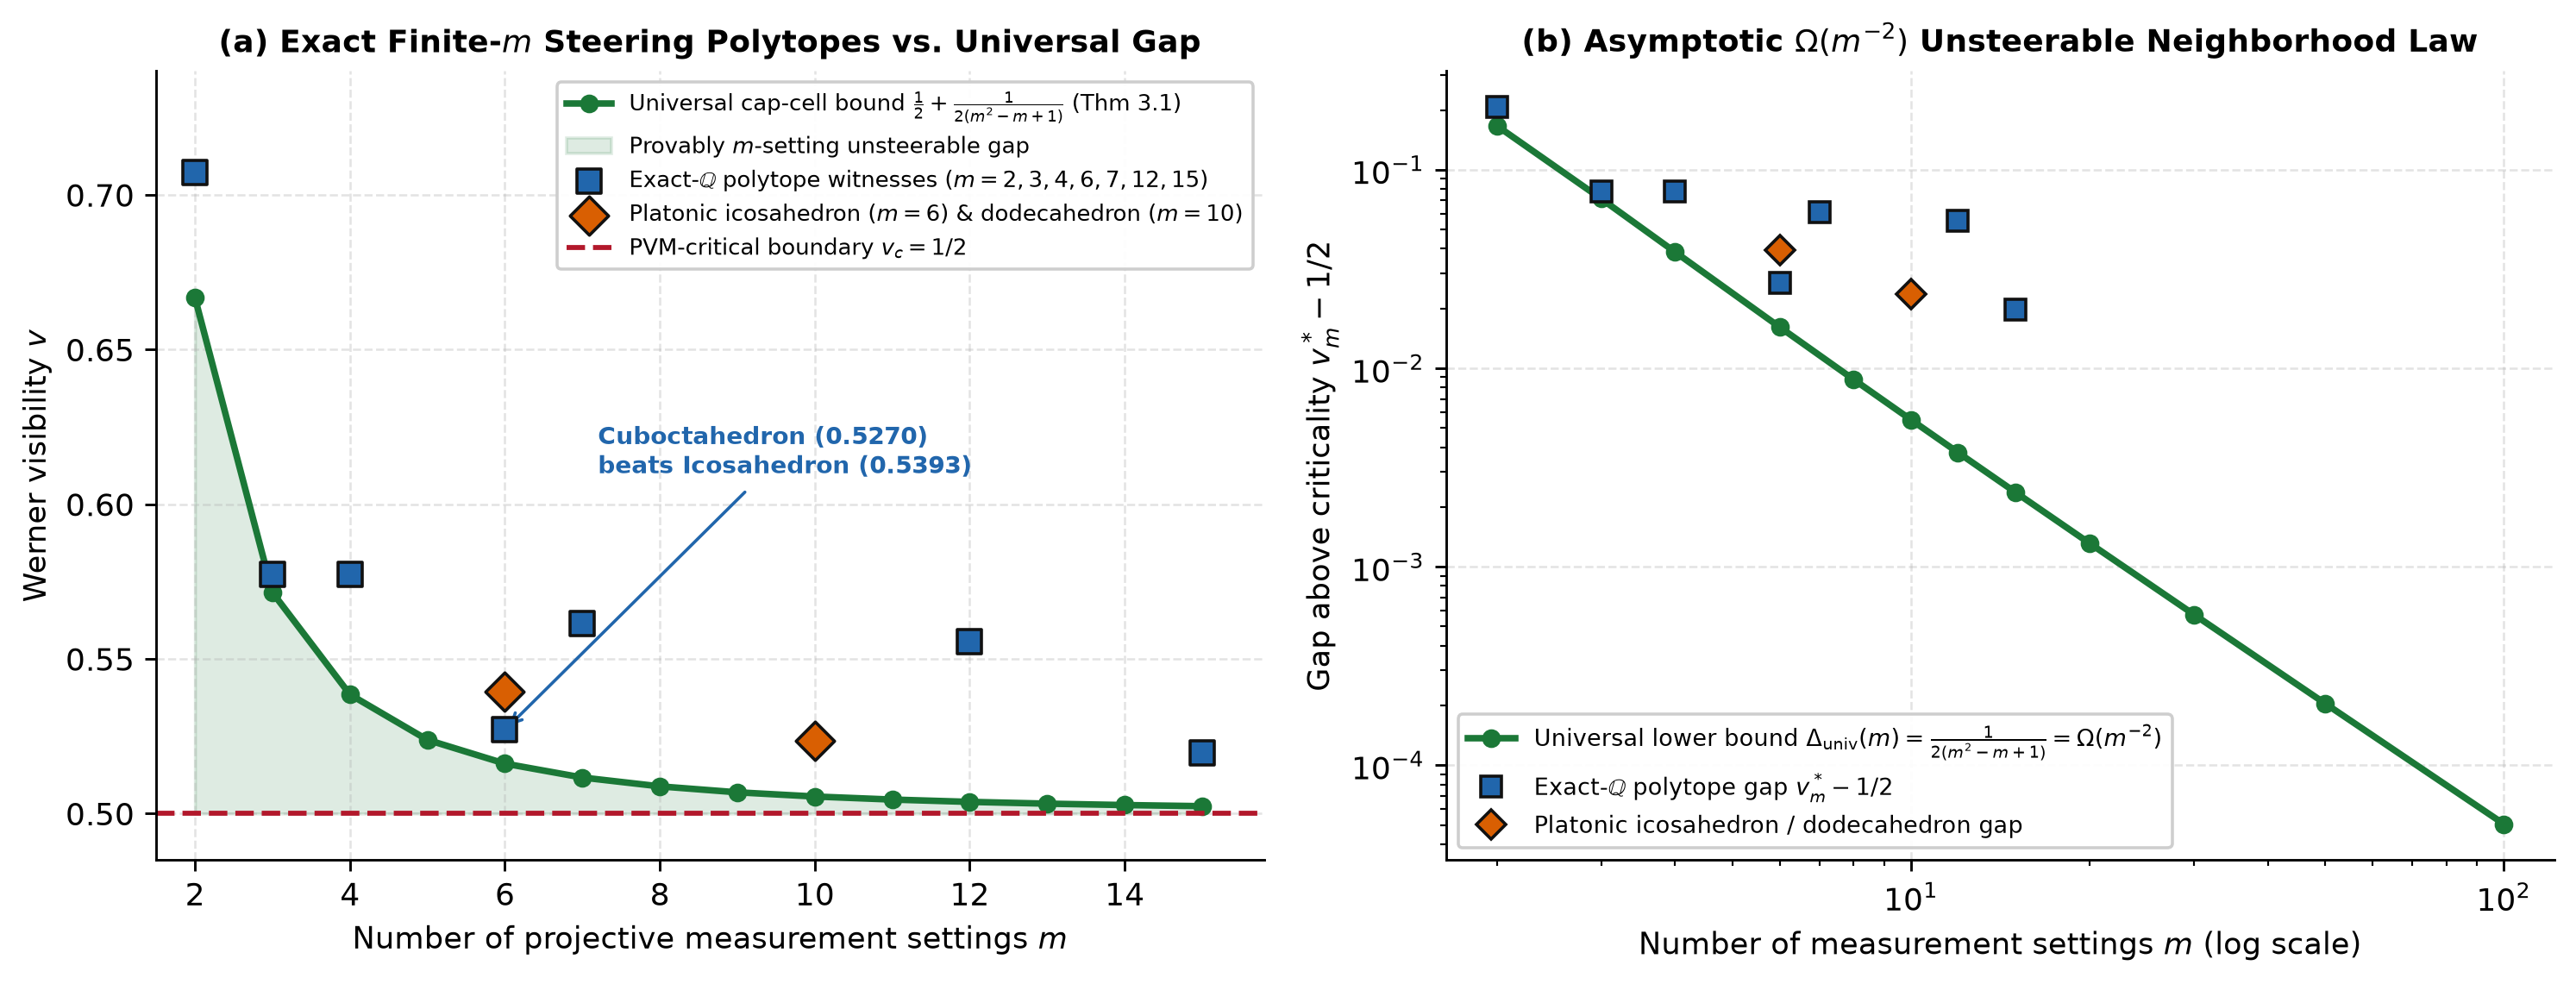
\includegraphics[width=\textwidth]{figures/fig1_finite_m_gap_and_polytopes.png}
\caption{Experiment~2: \textbf{(a)}~Exact finite-$m$ steering polytope thresholds ($m \in \{2,3,4,6,10\}$) and certified canonical-witness upper bounds $v_m^{\mathrm{can}} \ge v_m^*$ ($m \in \{7,12,15\}$) (squares: exact $\QQ$; diamonds: Platonic) versus Theorem~\ref{thm:univ-gap}'s universal cap-cell lower bound $v_{\mathrm{univ}}(m) = \frac{1}{2} + \frac{1}{2(m^2-m+1)}$ (green curve and shaded unsteerable region), highlighting cuboctahedral supremacy over the icosahedron at $m=6$. \textbf{(b)}~Log-log scaling of the gap above $v_c = 1/2$ confirming the non-asymptotic $\Omega(m^{-2})$ law up to $m=100$.}
\label{fig:polytopes}
\end{figure}

\paragraph{Experiments 3 \& 4: Haar Monte Carlo Cross-Check and Conditional-State PPT Phase Diagram.}
In Experiment~3, $100{,}000$ independent Haar $SO(3)\times SO(3)$ samples independently validate Theorem~\ref{thm:superact}: $\mathbb{E}_{S^2}[x^2 y^2 z^2] = 0.009492$ vs.\ exact $1/105 = 0.009524$ ($z = 0.96$); $L_{\mathrm{joint}}(0) = 0.68505 \pm 0.00069$ lies strictly below our exact-$\QQ$ SOS bound $5167/7056 \approx 0.73228 < 3/4$; and $L_{\mathrm{joint}}(q) \le \frac{5167}{7056} + \sqrt{2}\sin 2q$ holds across all $21$ Schmidt angles $q \in [0,\pi/4]$ (Figure~\ref{fig:superact}a). Sweeping $\gamma$ confirms that the tight continuous witness reaches $v_{\mathrm{tight}}^{(2)} \approx 0.4933 < 1/2$ at $\gamma = 3$, while our zero-float exact-$\QQ$ certificate crosses below $1/2$ analytically for all $\gamma > 7056/125 = 56.448$ (integers $\gamma \ge 57$; first plotted grid point $\gamma = 70$) and reaches $v_{\mathrm{cert}}^{(2)} \approx 0.499961 < 1/2$ at $\gamma = 114$ (Figure~\ref{fig:superact}b). In Experiment~4, all $40$ grid checks of~\eqref{eq:ppt-eigs} match direct $4\times 4$ matrix partial-transpose eigendecompositions to machine precision ($\max\text{err} = 1.11\times 10^{-16}$), mapping the exact PPT boundary $s_{\mathrm{swap}}(v) = (1-v^2)/(2v^2)$ (Figure~\ref{fig:ppt}a).

\begin{figure}[t]
\centering
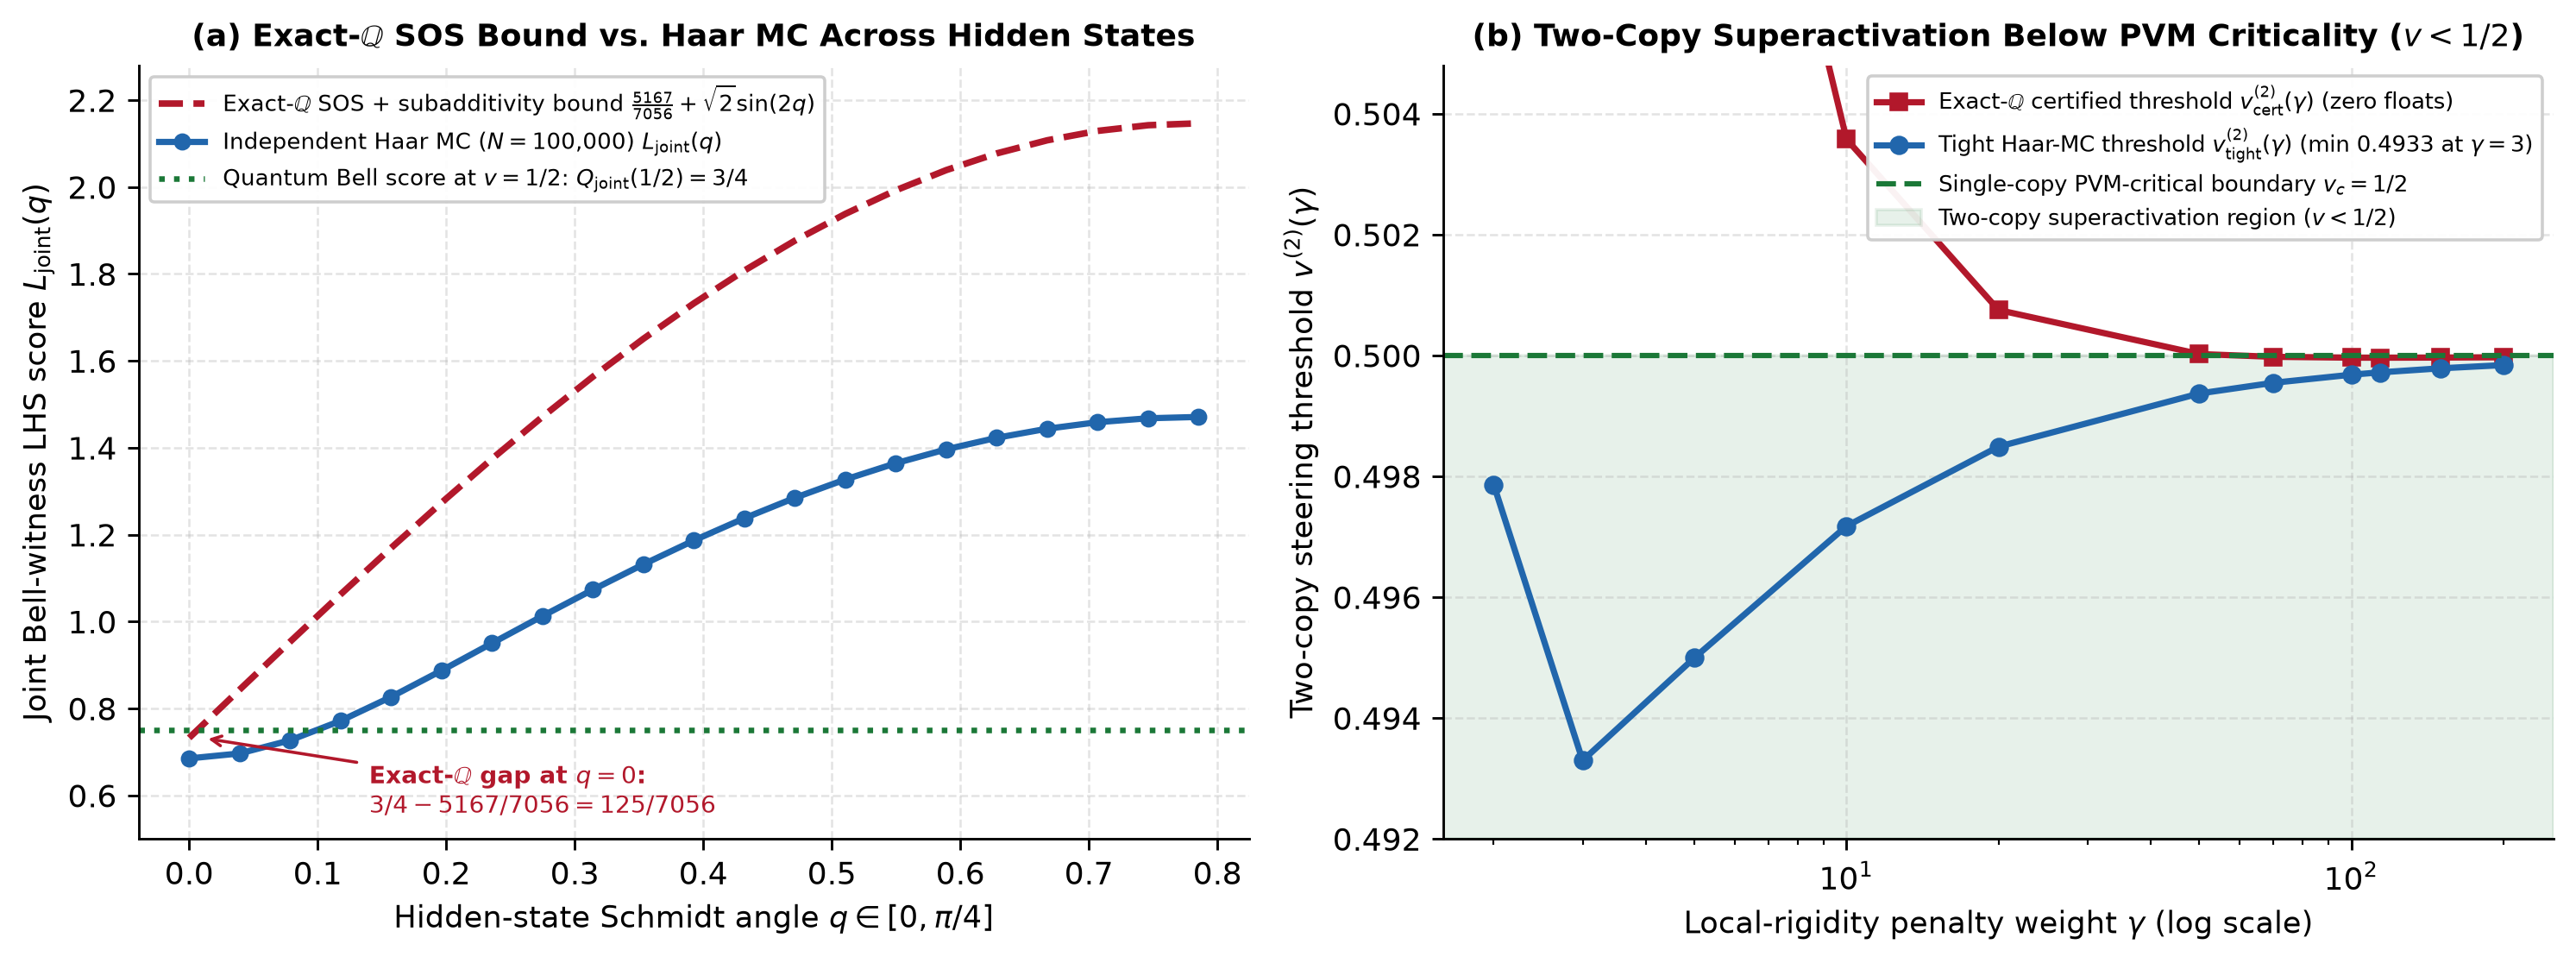
\includegraphics[width=\textwidth]{figures/fig2_two_copy_superactivation.png}
\caption{Experiment~3: \textbf{(a)}~Exact-$\QQ$ SOS + subadditivity upper bound $\frac{5167}{7056} + \sqrt{2}\sin(2q)$ (red dashed) strictly dominates $100{,}000$-sample Haar MC $L_{\mathrm{joint}}(q)$ (blue) across all two-qubit hidden-state Schmidt angles $q \in [0,\pi/4]$ while remaining strictly below $Q_{\mathrm{joint}}(1/2) = 3/4$ at $q=0$. \textbf{(b)}~Two-copy steering threshold $v^{(2)}(\gamma)$ crossing strictly below $v_c = 1/2$ both numerically ($0.4933$ at $\gamma=3$) and via zero-float exact-$\QQ$ certification ($\gamma \ge 57$ analytically, first plotted grid point $\gamma=70$, optimal $0.499961$ at $\gamma=114$).}
\label{fig:superact}
\end{figure}

\begin{figure}[t]
\centering
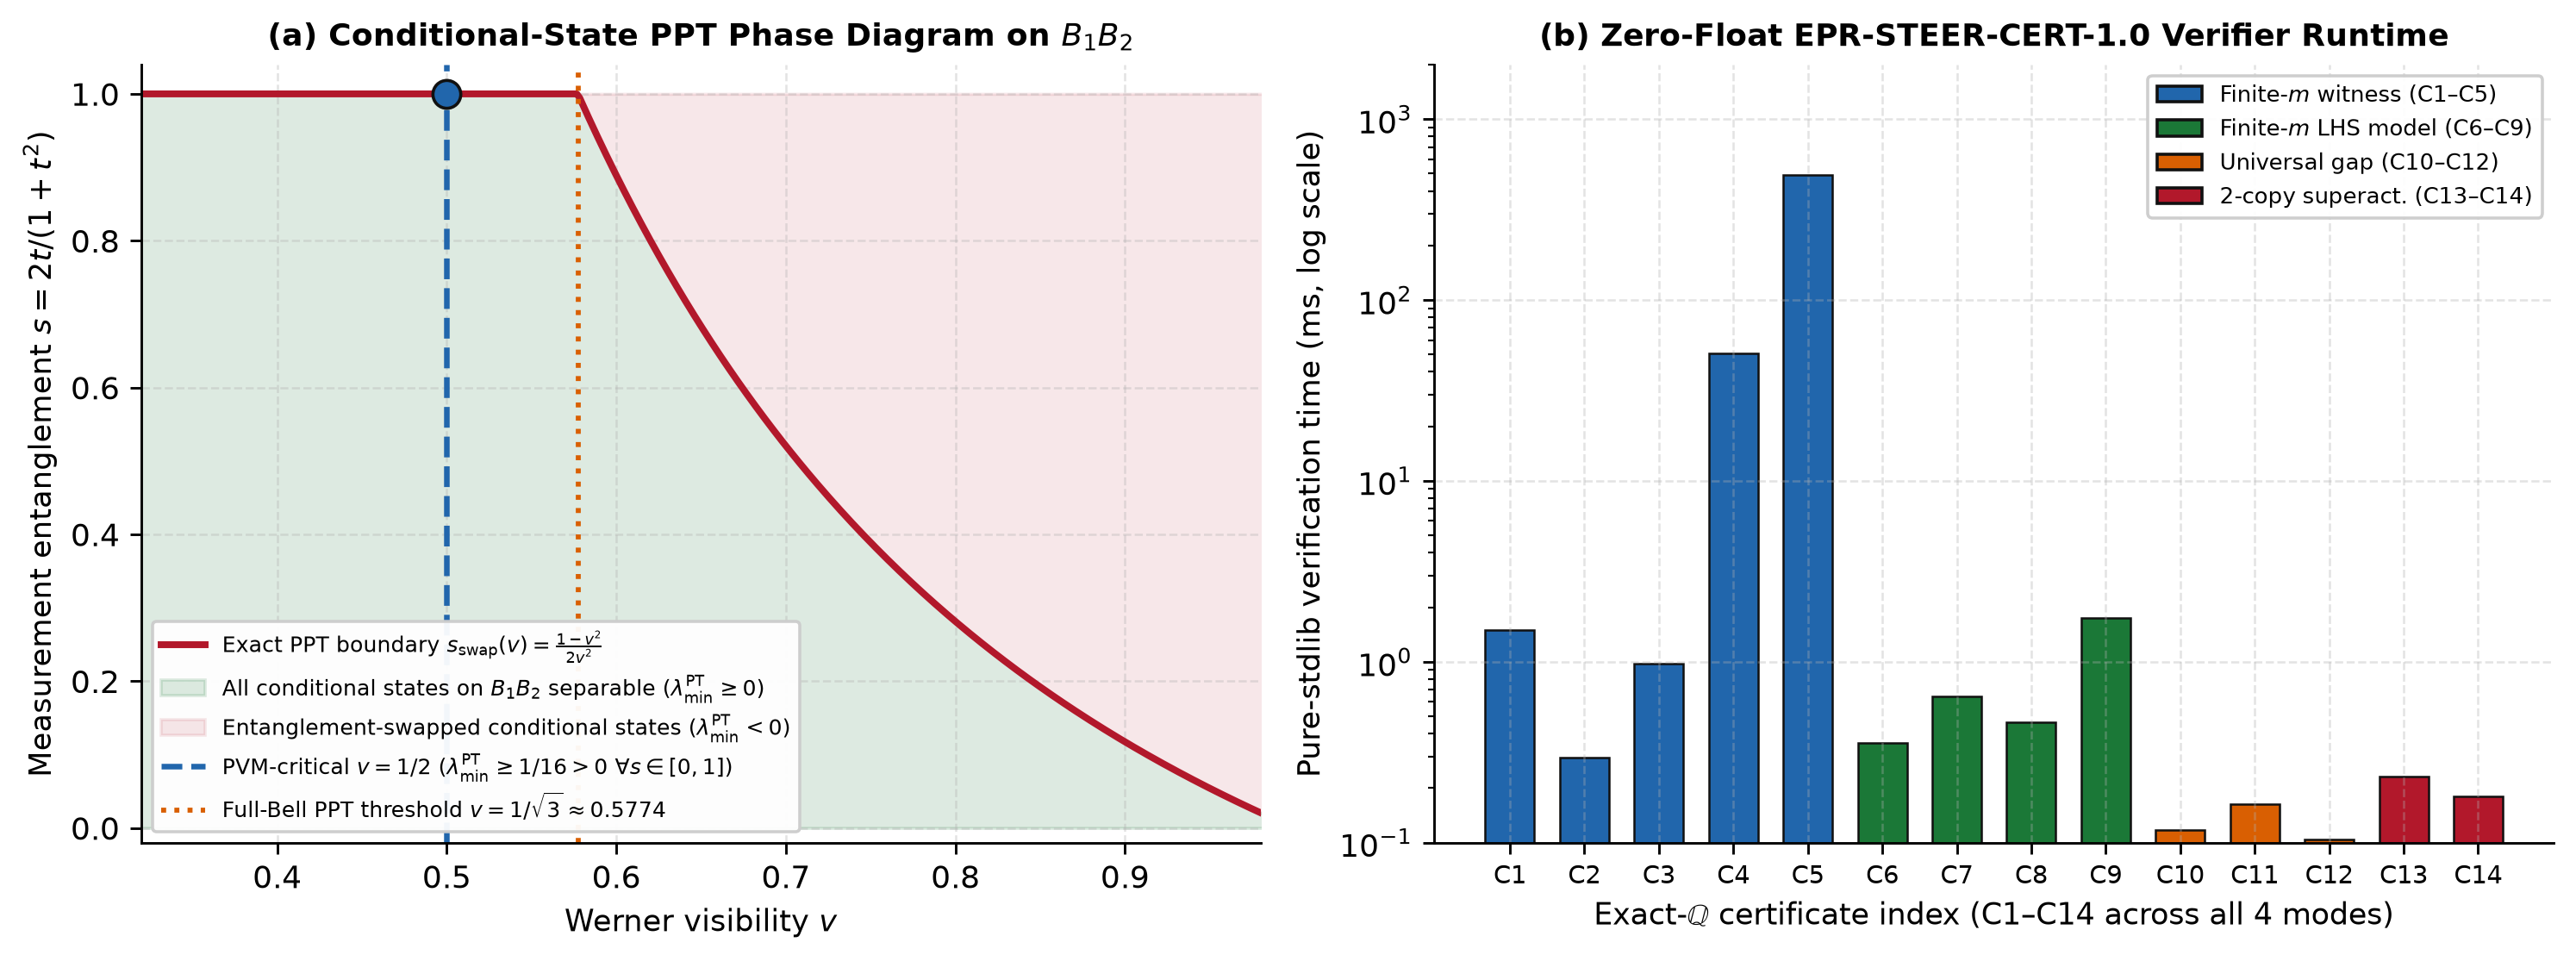
\includegraphics[width=\textwidth]{figures/fig3_ppt_separability_pocket.png}
\caption{Experiments~1 \& 4: \textbf{(a)}~Exact conditional-state PPT separability phase diagram on Bob's two qubits $B_1 B_2$ showing $s_{\mathrm{swap}}(v) = (1-v^2)/(2v^2)$ (red) and strict interior separability $\lambda_{\min}^{\mathrm{PT}} \ge 1/16 > 0$ along the entire PVM-critical line $v=1/2$ (blue dashed). \textbf{(b)}~Pure-stdlib \certschema{} verifier runtime (log scale) across all $14$ certificates (C1--C14).}
\label{fig:ppt}
\end{figure}

\paragraph{Adversarial Red-Team Verification ($46/46$ Attacks Rejected).}
The automated suite \texttt{tests/test\_suite.py} subjects \texttt{verify\_steering\_\allowbreak certificate\_\allowbreak exact} to $46$ live forgery attempts spanning schema, type, and identifier tampering, canonical rational parser bypasses, unviolated or forged witnesses, duplicate or antipodal axes, Bloch-ball violations ($\|\mathbf{b}\|_2^2 > N_u$), non-isotropic Bob marginals, non-uniform Alice marginals ($\sum p_\lambda a_x^{(\lambda)} \ne 0$), probability-sum violations, universal-bound violations, forged Bell constants, already single-copy steerable fake superactivation ($v = 11/20 > 1/2$), and non-PPT conditional states ($v=3/5$ with $\lambda_{\min}^{\mathrm{PT}} = -1/50$). All $46/46$ attacks raise \texttt{ValueError}.

\section{Discussion and Limitations}

Our results provide exact rational witnesses and machine-checked proofs for both sides of Zhang and Chen's critical EPR steering picture~\cite{zhang2026critical}: every finite-$m$ protocol is bounded away from $v_c = 1/2$ by at least $\frac{1}{2(m^2-m+1)}$, while two copies $\rho_v^{\otimes 2}$ unconditionally superactivate at and strictly below $v = 1/2$ with strictly separable conditional states.

Two limitations point to natural extensions. First, our exact-$\QQ$ two-copy superactivation witness uses the maximally entangled Bell measurement ($t=s=1$) rather than arbitrarily weak measurement entanglement ($t \to 0^+$), and targets the isotropic Werner boundary rather than general anisotropic Bell-diagonal states; extending our SOS-moment technique to arbitrarily small $t > 0$ and general $T$-states~\cite{jevtic2015einstein} is a compelling next step. Second, exhaustive sign-pattern verification in \texttt{finite\_m\_steering\_witness} scales as $O(2^{m-1})$ ($0.49$\,s at $m=15$); certifying larger $m \ge 20$ polytopes will benefit from symmetry-orbit reduction or exact branch-and-bound zonotope certificates.

\bibliographystyle{plain}
\bibliography{references}

\end{document}
